\chapter{Add-on A}
\label{fsms_repository}
\section{Usage}
\\
The newest version of FSM comparison may be found in doc/fsms.pdf. \\
All results may be found in doc/fsms\_results.pdf
\\
\\
To run tests and generate results:\\
\textit{make}\\

\newpage
\section{FAQ}

How to emulate super state behavior using nested fsm ?\\
Everything which might be designed using super state may be also done using nested fsm functionality.
For sure it's way of design/framework what will be chosen. Nevertheless using nested fsm
to emulate super state behavior is pretty easy.

\begin{figure}[htbp]
    \centering
    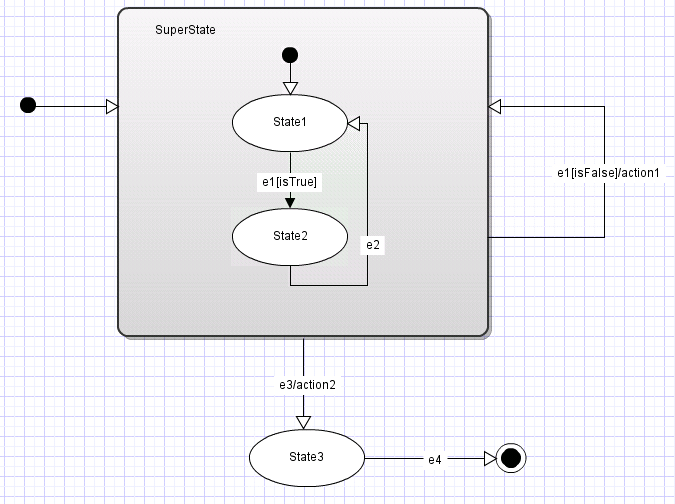
\includegraphics[scale=0.8]{images/faq/superstate.png}
    \caption[Super state]{Super state}
\end{figure}

\lstinputlisting{faq/superstate.hpp}

\newpage
How to dispatch non typed data to type safe fsm ?\\

\lstinputlisting{faq/dispatch.hpp}

